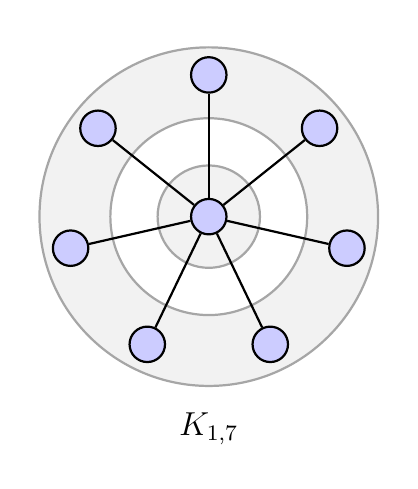
\begin{tikzpicture}[
  baseline=0pt,
  scale=1,
  vnode/.style={circle, draw=black, fill=blue!20, thick, inner sep=0pt, minimum size=4.5mm},
  edge/.style={thick, draw=black}
]
  \useasboundingbox (-2.3,-3.1) rectangle (2.3,2.4);

  % Partición 2 (Venn): Anillo exterior que encierra los 7 vértices
  \draw[thick, draw=gray!70, fill=gray!10, even odd rule] (0,0) circle (2.15cm) (0,0) circle (1.25cm);

  % Partición 1 (Venn): Círculo central que encierra el vértice central
  \draw[thick, draw=gray!70, fill=gray!10] (0,0) circle (0.65cm);

  % Vértice de la Partición 1 (Centro)
  \node[vnode] (a1) at (0, 0) {};

  % Vértices de la Partición 2 (7 vértices distribuidos uniformemente)
  \foreach \j in {1,...,7} {
    \pgfmathsetmacro{\ang}{90 + (\j-1)*360/7}
    \node[vnode] (b\j) at (\ang:1.8) {};
  }

  % Aristas desde el centro a cada vértice exterior
  \foreach \j in {1,...,7} {
    \draw[edge] (a1) -- (b\j);
  }

  % Etiqueta inferior
  \node[font=\large] at (0,-2.7) {$K_{1,7}$};
\end{tikzpicture}
